\documentclass{standalone}
\usepackage[utf8]{inputenc}
\usepackage{tikz,pgf}
\usepackage{amsmath}
%\usetikzlibrary{matrix,shapes.geometric,arrows,positioning,chains}
\usetikzlibrary{shapes.geometric,arrows}
\usetikzlibrary{calc}
\usepackage{relsize}

\tikzset{fontscale/.style = {font=\relsize{#1}}}

% Define the shapes to be used for the blocks
\tikzstyle{rectbox} = [rectangle, rounded corners, inner sep=4pt, 
 text width=11cm, draw = black, fill = blue!30]

 \tikzstyle{rectbox1} = [rectangle, rounded corners, inner sep=4pt, 
 text width=11cm, draw = black, fill = green!30]

\tikzstyle{rectbox2} = [rectangle, rounded corners, inner sep=4pt, 
 text width=6cm, draw = black, fill = blue!30]

\tikzstyle{decision} = [diamond,  
draw = black, fill = red!30, inner sep=0pt]

\tikzstyle{arrow} = [thick, ->, >=stealth]

\begin{document}

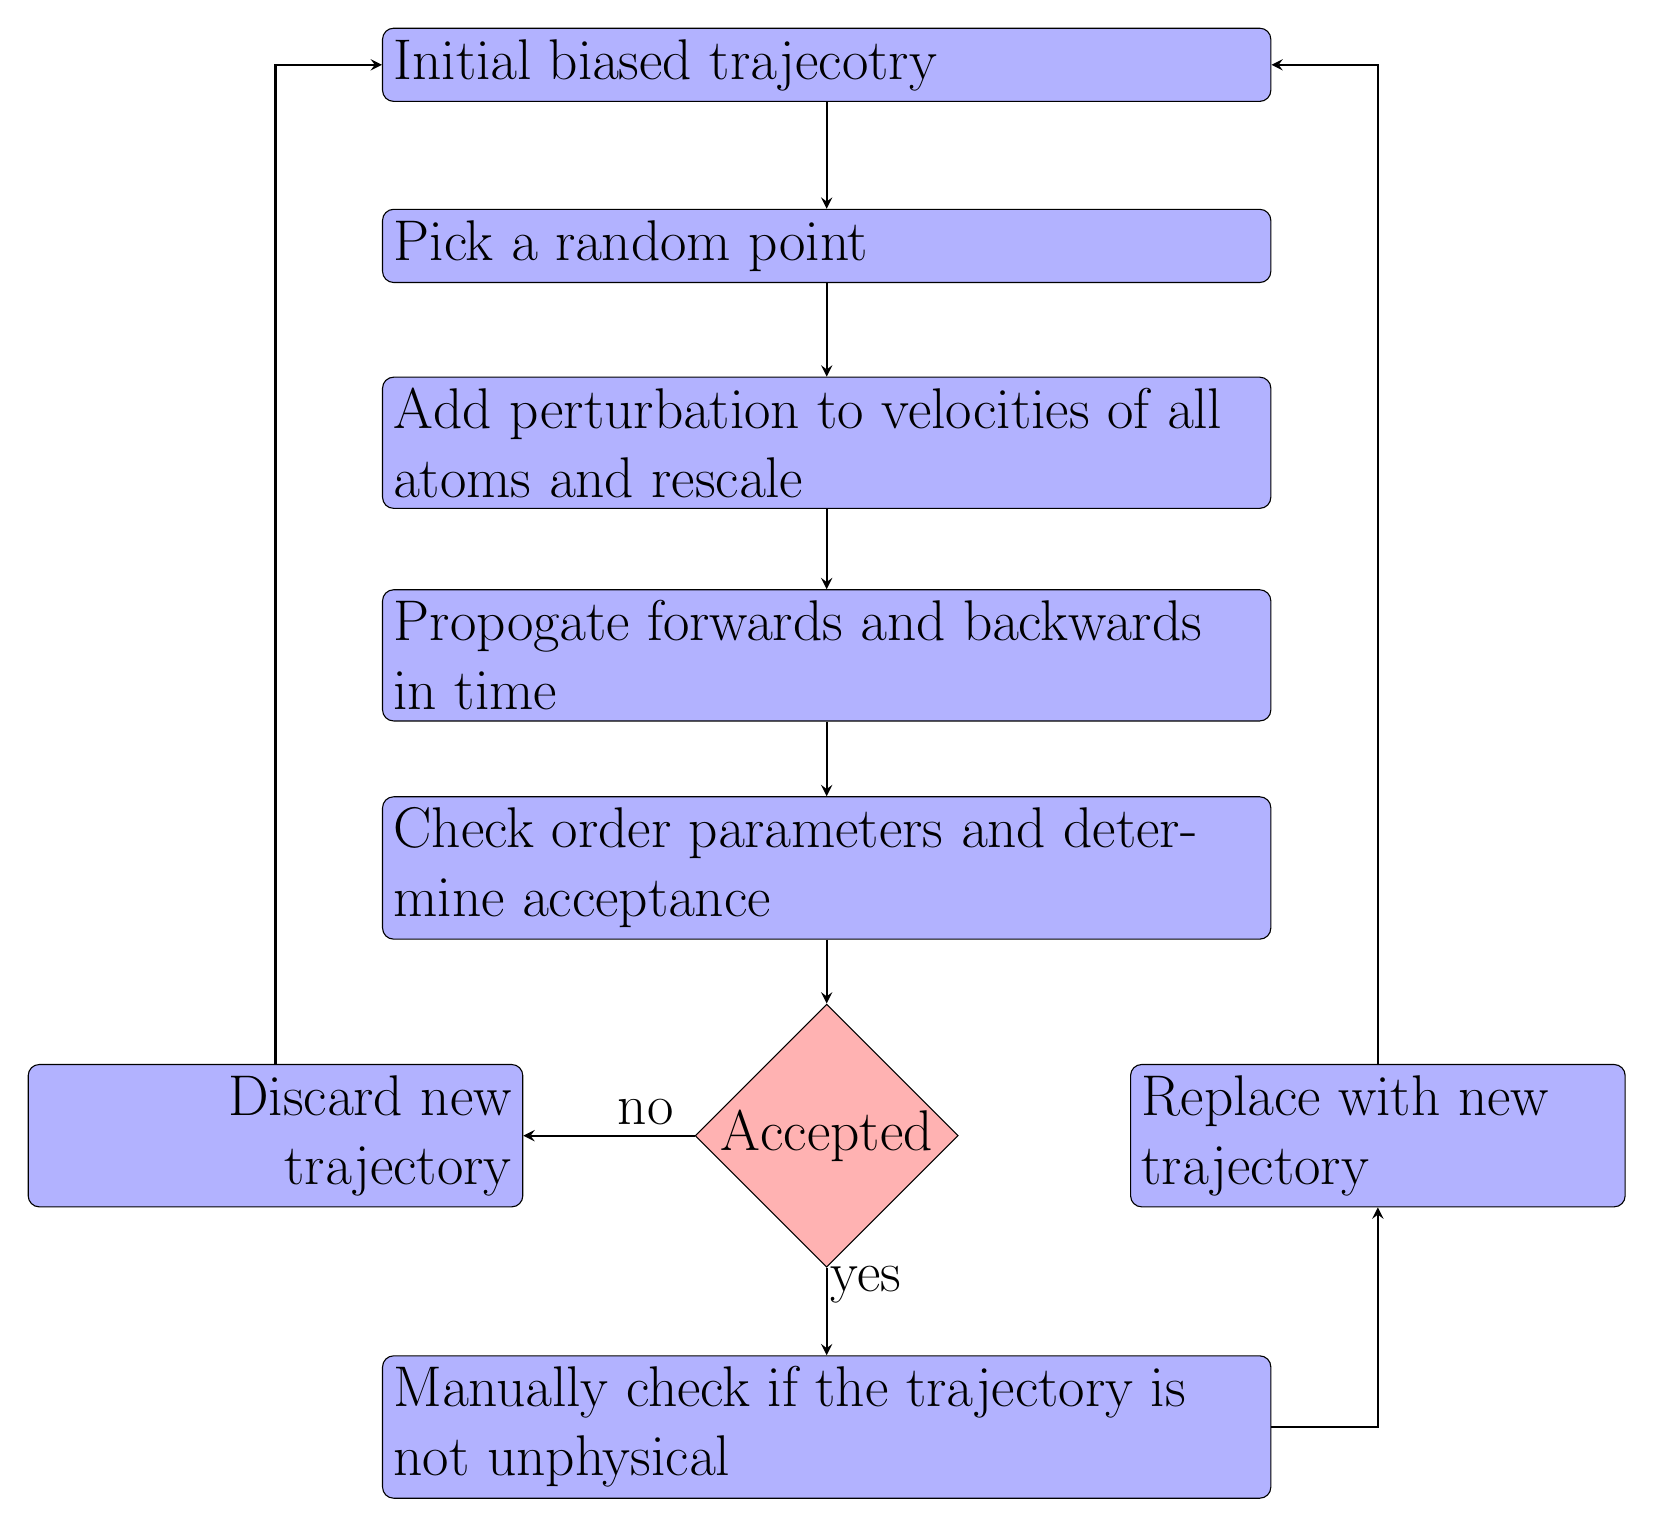
\begin{tikzpicture}[inner sep=1mm]

\node (start) [rectbox, fontscale=4.0] {Initial biased trajecotry};
\node (s1)    [rectbox, below of=start,yshift=-1.3cm, fontscale =4.0] {Pick a random point};
\node (s2)    [rectbox, below of=s1,yshift=-1.5cm, fontscale = 4.0] {Add perturbation to velocities of all atoms and rescale};
\node (s3)    [rectbox, below of=s2,yshift=-1.7cm, fontscale = 4.0] {Propogate forwards and backwards in time};
\node (s4)    [rectbox, below of=s3,yshift=-1.7cm, fontscale = 4.0] {Check order parameters and determine acceptance};
\node (s5)    [decision,below of=s4,yshift=-2.4cm, fontscale = 4.0] {Accepted};
\node (s8)    [rectbox, below of=s5,yshift=-2.7cm, fontscale = 4.0] {Manually check if the trajectory is not unphysical};
\node (s6)    [rectbox2,right of=s5, xshift=6.0cm, fontscale = 4.0] {Replace with new trajectory}; 
\node (s7)    [rectbox2, left of=s5,xshift=-6.0cm, align=right, fontscale = 4.0] {Discard new trajectory};
%\node (s5)    [rectbox, right of=s4] {Input orbitals}

\draw [arrow] (start) -- (s1);
\draw [arrow] (s1) -- (s2);
\draw [arrow] (s2) -- (s3);
\draw [arrow] (s3) -- (s4);
\draw [arrow] (s4) -- (s5);
\draw [arrow] (s5) -- node[anchor=south, fontscale=4.0, xshift=0.5cm] {yes} (s8);
%\draw [arrow] (s5) -- node[anchor=east, fontscale = 4.0] {yes} (s6);
\draw [arrow] (s5) -- node[anchor=west, fontscale = 4.0, yshift=0.3cm] {no} (s7);
%\draw [arrow] (s6) |- (start);
\draw [arrow] (s7) |- (start);
\draw [arrow] (s8) -| (s6);
\draw [arrow] (s6) |- (start);
\end{tikzpicture}

\end{document}
